\documentclass[a4paper, 12pt]{article}
%\documentclass[a4paper, 12pt, draft]{article} % don't include images, leave a border of same size...great
%\documentclass[journal]{IEEEtran}



%\usepackage[cmex10]{amsmath, mathtools}
\usepackage{amsmath,amssymb,amsbsy,amsfonts,amsthm}
\usepackage{multirow}
\usepackage{bm}
\usepackage{enumerate}
\usepackage{url}
\usepackage[ruled,vlined]{algorithm2e}
\usepackage{fancyvrb}
\usepackage{yfonts}

\usepackage{wrapfig}
\usepackage{tikz}
%\input{../tikz.conf}

\usetikzlibrary{bayesnet}

%%%%%%%%%%% Box 
\usepackage{calc}%    For the \widthof macro
\usepackage{xparse}%  For \NewDocumentCommand
\newcommand{\tikzmark}[1]{\tikz[overlay,remember picture] \node (#1) {};}


%\input{./header.tex}
%%%%%%%%%% Math
\renewcommand{\text}{\textnormal}
%\newcommand{\pr}{\mathbf{p}}
\newcommand{\pr}{p}
\newcommand{\p}{p}
\newcommand{\E}{\mathbb{E}}
\newcommand{\divkk}{\mathbb{K}}
\newcommand{\entropy}{\mathbb{H}}
\newcommand{\gem}{\mathrm{GEM}}
\newcommand{\Mult}{\mathrm{Mult}}
\newcommand{\DP}{\mathrm{DP}}
\newcommand{\IBP}{\mathrm{IBP}}
\newcommand{\M}{\mathcal{M}}
\newcommand{\V}{\mathcal{V}}
\newcommand{\N}{\mathcal{N}}
\newcommand{\h}{\mathcal{H}}
\newcommand{\mat}[1]{\mathbf{#1}}
\newcommand{\unit}{1\!\!1}

%\renewcommand{\Phi}{\mat{\Phi}}

\title{Mixed-Membership Inference in Sparse Weigted Networks.}

%\date{avril 2015}

\newtheorem{definition}{Definition}[section]
\newtheorem{proposition}{Proposition}[section]
\newtheorem{theorem}{Theorem}[section]
\newtheorem{corollary}{Corollary}[section]

\begin{document}
	
\maketitle
\begin{abstract}
\end{abstract}



\section{Introduction}

Relational data is widespread in many modern applications. From social networks to protein interactions, from physics to linguistics, all interacting objects can be represented as a graph where the objects are the nodes and the interactions the edges. The interest for modelling such networks has naturally increased with the availability of large datasets. Especially in the machine learning literature, that focused on link prediction, dimensionality reduction and data exploration tasks. One of the main challenge in this area is to be able to handle massive networks that emerge from the web. In this paper, we focus on networks that underpin some kind of social relationship such as collaboration or communication networks. In this context, we propose an online learning algorithm that we derived for both binary and count edge covariate, within the framework of Mixed-Membership Stochastic Blockmodel (MMSB).

%%% The type of networks that exists
%Complex networks are graphs that are used to represents real world relationnal information. In computer science, a major network is the web that connects a large amount of data. There is a large diversity in the type of data that can be interconnected, which ca be a set of people in a social plateform, a set of documents linked with hyperlinks, communication networks of email  or more recently a graph of transaction encoded in a blockchain. Outside the web an other important networks is the one made of the scientific collaborations.

%%% The Scalability problem => Sparse Network E/N**2 << 1
%The complexity (time and memory) of batch algorithm are polynomial for graph. Thus, the need of online algorithm, able to update a model as data become available is fundamental for scaling strategy. This can because of the temporality of the data or more simply because the data don't fit in memory. Another source of diversity in networks is the support for labelled and dynamic networks. In this paper we study and propose an algorithm based on latent models with rich priors who scale for complex and massive networks, with labeled edges (weighted networks), and that can be adapted to model the exchangeability of sequences of binary networks (temporal networks).


\section{Weighted Networks or Time exchangeability}

% dense - unrealistic
The link prediction models, in the literature \cite{review1,review2}, usually represents networks by a graph $G=(V,E)$ where the edges in the set $E$ are either $0$ or $1$ to account respectively for the absence or the presence of an edge between two nodes. Formally the likelihood of such model is characterized by a Bernoulli density such that $y_{ij} \sim \mathrm{y_{ij} |\theta_{ij}}$. Moreover all of those models are in a setting of static graphs which is formally traduced by the assumption of exchangeability. It means that the joint probability of a graph do not depend on the order of which we observes the nodes. %? $echangeability$

% sparse - real
The main limitation of such models is that they can't handle sparse networks, which is a corollary of the Aldous-Hoover theorem \cite{orbanz2015bayesian}. The models has been said to be misspecified. A way to alleviate this limitation is to weight edges instead of considering binary one. This weighting can be understood, in some way, as smoothing the networks. Additionally, a weighted network is a binary networks where information has bee added under the for of node labeling. The reason why sparsity could be handle this way is because, by considering a weighted networks, it makes all non-edges in a network (0 entries in the adjacency matrix) having a weak contribution to the degree distribution of associated node (see section \ref{todo}). Thus, the inference process can take advantage of this fact because, in sparse networks, most of the interactions are unrealized.

In this paper we will consider the weighted relations as a measure for the number of times each nodes have interacted. Thus, a natural prior for such assumptions is a Poisson distribution. It follows that we will define the likelihood to generate a weighted edge such that $y_{ij} \sim \mathrm{\theta_{ij})}$. Moreover, this representation can take advantage of relational data that arise in various scenario, summarized by the two following:
\begin{itemize}
\item Weighted Networks, where weights represent the \emph{strength} of the relations between individuals,
\item Sum of \emph{snapshot} of binary (or weighted) networks.
\end{itemize}

In the second case the weights can also be seen as a \emph{strength} of connection between individuals, since it represents a count/number of times they interacted together. There is a number of situations where such a case arise. One can think for example to the count of clicks that one user makes during a session. Or the number of time that a individual send a message to another in a social network or again the number of transportation between two cities. Thus modeling weighted networks is a way to take into account the strength of relations that arise in a temporal context, but by keeping the exchangeability assumptions. Or say differently, we loose the time order in which each individual connections took place. That is the reason why we use the term \emph{time exchangeability}.

The use of a Poisson law as an aggregator for single snapshots is primarily justified by the two following fundamental properties \cite{orbanz2012lecture}:
\begin{itemize}
\item{Additivity}: If $K_1 \sim \mathrm{Poisson}(\alpha_1)$ and $K_2 \sim \mathrm{Poisson}(\alpha_2)$ then:
    \begin{equation}
        K_1 + k_2 = \mathrm{Poisson}(\alpha_1 + \alpha_2)
    \end{equation}
\item {Thinning}: The number of successes in a Poisson number of coin flips is Poisson, namely if $K \sim \mathrm{Poisson}(\alpha)$ and $X_1,...,X_2 \sim_{iid} \mathrm{Bern}(p)$, then:
    \begin{equation}
        \sum_{i=1}^K X_i = \mathrm{Poisson}(p\alpha)
    \end{equation}
\end{itemize}

Those two properties of the Poisson distribution constitute the justification of building weighted networks datasets from sequence of either weighted graphs or binary graphs and making inference with Poisson based likelihood.

\section{Model -- WMMSB}
A powerful model for binary exchangeable networks is the Mixed Membership Stochastic Blockmodel (MMSB). In order to keep the strength behind the MMSB models, we propose a generalization of it for weighted networks such as described in the previous section.

The proposed model is a weighted extension of MMSB, named WMMSB. The main design difference is that the likelihood is drawn from a Poisson distribution, and the correlations between the shared classes are drawn from independent Gamma distribution. The models first draw latent class membership for each nodes from a shared Dirichlet distribution. Then for each interactions, each node draw a single membership. The observation level is then draw from Poisson distribution taking is rate parameter according to two classes that summarize the interaction between the two underlying nodes. The observation corresponds to the strength of the relationship. The generative model (along  with the graphical model) is summarized as follows:

\begin{figure}[h]
\begin{minipage}[h]{0.45\linewidth}
\begin{align*}
	&\textrm{For each } i \in \{1, .., N\}  \\
	&\qquad\bm{f}_i \sim \textrm{Dir}(\alpha)\\
	&\textrm{For each }  (m,n) \in \{1,..,K\}^2 \\
	&\qquad\phi_{mn} \sim \mathrm{Gamma}(k,\theta)\\
	&\textrm{For each } (i,j) \in V^2 \\
	&\qquad z_{i \rightarrow j} \sim \mbox{Cat}(\bm{f}_i)\\
	&\qquad z_{i \leftarrow j} \sim \mbox{Cat}(\bm{f}_j)\\
    &\qquad y_{ij} \sim \mathrm{Poisson}(\phi_{z_{i \rightarrow j}z_{i \leftarrow j}})
\end{align*}
\end{minipage}
\begin{minipage}[h]{0.45\linewidth}
	\scalebox{0.88}{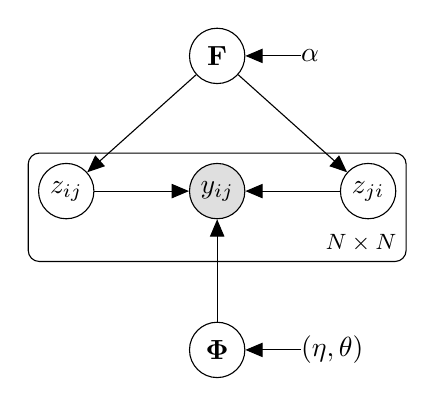
\begin{tikzpicture}
    %\begin{scope}[yshift=0.5cm]
  % Define nodes
  \node[obs]                      (y) {$y_{ij}$};
  \node[latent, left=1.2cm of y] (zi) {$z_{ij}$};
  \node[latent, right=1.2cm of y] (zj) {$z_{ji}$};
  \node[latent, above= of y]    (ibp) {$\mat{F}$};;
  \node[latent, below= of y, yshift=-0.3cm]   (W) {$\mat{\Phi}$};
  \node[const, right=0.7cm of ibp]   (b) {$\alpha$};
  \node[const, right=0.7cm of W]   (sw) {($\eta,\theta$)};

  % Connect the nodes
  \edge {zi,zj,W} {y} ;
  \edge {ibp} {zi,zj} ;
  \edge {sw} {W} ; 
  \edge {b} {ibp} ; 

  % Plates
  \plate {yx} {(zj)(zi)(y)} {$N\times N$} ;
  %\end{scope}
\end{tikzpicture}
}
\end{minipage}
    \caption{Generative models and Bayesian graph of WMMSB.}
\end{figure}

Note that the group membership of each node is context dependent. That is, each node may assume different membership when interacting or being interacted with by different peers. Statistically, each node is an admixture of group-specific interactions. The two sets of latent group indicators are denoted by $\{z_{p\rightarrow q} : p, q \in V\}  =: Z_\rightarrow$ and $\{z_{p\leftarrow q} : p, q \in V\}  =: Z_\leftarrow$. Also note that the pairs of group memberships that underlie interactions need not be equal; this fact is useful for characterizing asymmetric interaction networks. Equality may be enforced when modeling symmetric interactions. \ref{goldenberg2010survey}.

%In the rest of this paper  we will note the set of hyperparameters as $\H = (\alpha, \theta, k)$.

For simplicity, the marginal likelihood (or evidence), takes the following form:
\begin{equation}
    \p(Y | \alpha, \Phi) = \int_F \sum_Z \p(Y| Z, \Phi) \p(Z|F) \p(F| \alpha) dF
\end{equation}

Furthermore, observed links are conditionally independant given the parameters for nodes ($F$) and for classes ($\Phi$) and by marginalizing over the class membership. Thus the likelihood can be written as a matrix decomposition :
\begin{equation}
P(Y | F, \Phi) = \prod_{i,j \in V^2} f_i \Phi f_j^T
\end{equation} 

Unfortunately the evidence is intractable, and conducts the practitioner to resort to approximate inference. In the next section, we propose a Stochastic Collapsed Variationnal inference method.

\section{Inference}

\textcolor{red}{Erics/Chrsitine Note's : Until the double column below wich deal with both network models type, weighted and binary (poisson/bernoulli), the variational derivation holds for both. Just the structure of the Bayesian Graph matter, the familly of the parameter's distribution does not. Furthermore, if the familly distribution of parameters falls into the exponential familly wth conjugate prior, there is closed form updates for the variational inference.}

The Variational Baye's (VB) method is an inference method where the parameters of the Bayesian model, $(F, \Phi, Z)$, are approximated with some free variational parameters $(\nu, \epsilon, \gamma)$. It consists of an iterating algorithm which updates the variational parameters. Those updates are found by maximizing the lower bound arising from the Jensen Inequality. This is equivalent to  minimize the Kullback-Leibler divergence between the variational (posterior) distribution over the variational parameters denoted $q(F, \Phi, Z | \nu, \epsilon, \gamma)$ (we will suppress reference to the variational parameters in the variational posterior for brevity) and the true (posterior) distribution $p(F, \Phi, Z | \tau)$ where $\tau = (\alpha, k, \theta)$ denotes the set of hyperparameters of the model. The evidence lower bound (ELBO) takes the following form :

\begin{equation}
\log p(Y | \tau) = \mathcal{L}(q(F, \Phi, Z)) \geq E_q[\log p(Y, F, \Phi, Z | \tau)] + E_q[\log q(F, \Phi, Z)]
\end{equation}

In classical VB, the variational parameters are taken in the same familly of the true parameters and by assuming that they are fully independent such that :
\begin{equation}
q(F, \Phi, Z) = \prod_{i\in V}q(f_i | \nu_i) \prod_{k,k' \in K^2}q(\phi_{kk'} | \epsilon_{kk'})\prod_{i,j \in V^2}q(\zij, \zji | \gamma_{ij})
\end{equation}

In the Collapsed Variational Baye's (CVB), the assumption on the variational distribution is much weaker. We only assume that the $Z$ variables are mutually independent, thus the variational posterior becomes : 
\begin{align}
q(F, \Phi, Z) &= q(F,\Phi) \prod_{(i,j)\in V^2}q(\zij, \zji | \gamma_{ij}) \\
	&= q(F, \Phi | Z)q(Z)
\end{align}

The ELBO can be split by separating both independent contributions of the variational posterior. Since we do not restrict the form of $q(F, \Phi | Z)$, the ELBO maximum is achieved when the true posterior is reached at $p(F, \Phi | Y, Z,  \tau) = q(F, \Phi | Z)$. The ELBO simplifies in the following collapsed form :
\begin{equation}
\mathcal{L}(q(Z)) = \max_{q(F,\Phi|Z)} \mathcal{L}(q(F, \Phi|Z)q(Z)) = E_q[\log p(Y,Z|\tau)] - E_q[q(Z)]
\end{equation}

The variational parameters are chosen in the same family than the true distribution, thus $q(\zij=k, \zji=k' | \gamma_{ij})$ are multinomial with parameters $\gamma_{ijkk'}$.

Finally, the CVB updates are obtained by minimizing the collapsed ELBO with respect to $\gamma_{ijkk'}$ and it takes the following general form :
\begin{equation} \label{eq:cvb_update}
    \gamma_{ijkk'} \propto \exp \left( E_{q(Z^{\neg ij})} [log(\zij=k, \zji=k' |Y, Z^{\neg ij}, \tau)] \right)
\end{equation}

Where the superscript $\neg ij$ means that the corresponding variables (or counts) are excluded.
This equation is not directly tractable, therefore it is possible to approximate equation \eqref{eq:cvb_update} by noting its relation with the collapse gibbs update. Then,  the closed form expression for the CVB update can be obtain by using a central limit theorem approximation followed by a Taylor expansion.



%\setlength{\columnseprule}{1pt}
%\def\columnseprulecolor{\color{blue}}
%\begin{multicols}{2}[]


The collapse Gibbs update for both models are given by the following equations :

\begin{itemize}
    \item Bernoulli Kernel (MMSB) : \[p(\zij=k, \zji=k' | Y, Z^{\neg ij}, \tau) \propto \quad \frac{ n^{\Phi\neg ij}_{y_{ij}kk'} + \lambda_{y_{ij}}}{n^{\Phi\neg ij}_{\bm{.}kk'} + \lambda_{\bm{.}}} (n^{F\neg j}_{ik} + \alpha_k) (n^{F\neg i}_{jk} + \alpha_{k'})\]
    \item Poisson Kernel (WMMSB) : \[p(\zij=k, \zji=k' | Y, Z^{\neg ij}, \tau) \propto \quad  NB(n^{\Phi\neg ij}_{y_{ij}kk'} + k, \widehat{n}^{\Phi\neg ij}_{y_{ij}kk'} + \theta ) (n^{F\neg j}_{ik} + \alpha_k) (n^{F\neg i}_{jk} + \alpha_{k'})\]
\end{itemize}

Where $NB(a, b)$ represents the pdf of a negative binomial distribution.

The collapse Gibbs Sampler only need to update the counts $n^{n^{\Phi\neg ij}}_{xkk'}, n^{F\neg j}_{ik}, n^{F\neg i}_{jk}$ and $x$ takes its support respectively in $(0,1)$ and $\mathbb{N}$ for MMSB and WMMSB.

In order to compute equation \eqref{eq:cvb_update}, one can approximate the variational distribution with a zero order Taylor expansion under a Gaussian approximation. This is know as the CVB0 algorithm, which gives the following updates :

\begin{itemize}
    \item MMSB : \[ \gamma_{ijkk'} \propto \quad \frac{ N^{\Phi\neg ij}_{y_{ij}kk'} + \lambda_{y_{ij}}}{N^{\Phi\neg ij}_{\bm{.}kk'} + \lambda_{\bm{.}}} (N^{F\neg j}_{ik} + \alpha_k) (N^{F\neg i}_{jk} + \alpha_{k'})\]
    \item WMMSB : \textcolor{red}{Todo}
\end{itemize}

    One can remark the similarity with the Collapse Gibbs update. The difference lives in the counts who now correspond to the means over the variational distribution $q$. The means are approximated trough the central limit theorem of the sum of independent Bernoulli variables with mean $\gamma_{ijkk'}$ such that :
\begin{itemize}
    \item $N^{\Phi}_{xkk'} = \sum_{ij:y_{ij}=x} \gamma_{ijkk'}  \approx   E_q[n^{\Phi}_{xkk'}] $
    \item $N^{F}_{ik}  =  \sum_{j, k'} \gamma_{ijkk'} \approx   E_q[n^{F}_{ik}]$
\end{itemize}


~\\
\textcolor{red}{To complete down here  : ~\\
SCVB update - presents algorithms with noisy gradients and stepsize, minibatch setc.
}



\section{Experiments}

%WMMSB compare it with LDA (a mask)i vs a bipartite networks (Document)
%D (doc) x W (Voc) -- entry count
%
%the bag of word VS the networks representation of document
%* it adds a parameter the document modelization !!!!!!!

\clearpage

\bibliographystyle{unsrt}
\bibliography{./a}

\appendix

\end{document}

